%   Journal Article Template
%%%%%%%%%%%%%%%%%%%%%%%%%%%%%%%%%%%%%%%%%%%%%%%%%%%%%%%%%%%%%%%%%%%%%%%%
\documentclass{article}
\usepackage{graphicx}
\usepackage{amssymb}
\usepackage{bm}
%\usepackage[notref,notcite]{showkeys}
%\usepackage[dvipdfm]{hyperref}
%\usepackage{hyperref}
\usepackage{graphicx}
%\usepackage{subfigure}
%\usepackage{epsfig,psfig}
\usepackage{amsfonts,amsmath,latexsym}
\usepackage{amsbsy}
\usepackage{nicefrac}
\usepackage{subcaption}
%%%%%%%%%%%%%%%%%%%%%%%%%%%%%%%%%%%%%%%%%%%%%%%%%%%%%%%%%s
%%%%%%%%%%%%%%%%%%%%%%%%%%%%%%%%%%%%%%%%%%%%%%%%%%%%%%%%%%%
%
% PROOF
%
%\newenvironment{rproof}{\addvspace{\medskipamount}\par\noindent{\it Proof:\/}}
%{\unskip\nobreak\hfill$\Box$\par\addvspace{\medskipamount}}
%
% ROMENUM
%

%
% special SYMBOLS
%
\newcommand{\uu}[1]{\boldsymbol #1}                     % vector fields
\newcommand{\uuu}[1]{\underline{#1}}                 % tensor fields
\newcommand{\jmp}[1]{[\![#1]\!]}                     % jump
\newcommand{\mvl}[1]{\{\!\!\{#1\}\!\!\}}             % mean value
%
% NORMS
%
\newcommand{\N}[1]{\|#1\|}                            % norm
\newcommand{\tn}[1]{|\!|\!|#1|\!|\!|}             % triple norm
%
\newcommand{\mc}[1]{\mathcal{#1}}
\newcommand{\curl}{\rm curl}
\newcommand{\dvr}{\rm div}
\newcommand{\nedelec}{N\'{e}d\'{e}lec }
\newcommand{\fenics}{{\tt FEniCS} }

\newcommand{\grad}{\ensuremath{\nabla}}
%
%%%%%%%%%%%%%%%%%%%%%%%%%%%%%%%%%%%%%%%%%%%%%%%%%%%%%%%%%%%%%%%%%%%%%%%%%%%%%%%%%%%%%%%%%%%%%%%%%
% end: our definitions
%%%%%%%%%%%%%%%%%%%%%%%%%%%%%%%%%%%%%%%%%%%%%%%%%%%%%%%%%%%%%%%%%%%%%%%%%%%%%%%%%%%%%%%%%%%%%%%%%%%


%\newenvironment{Pf}{\noindent {\bf Proof:}} {\hfill $\Box$ \medskip}
%
%%%%%%%%%%%%%%%%%%%%%%%%%%%%%%%%%%%%%%%%%%%%%%%%%%%%%%%%%%%%%%%%%%%%%%%%
%%%%%%%%%%%%%%%%%%%%%%%%%%%%%%%%%%%%%%%%%%%%%%%%%%%%%%%%%%%%%%%%%%%%%%%%






%
%%%%%%%%%%%%%%%%%%%%%%%%%%%%%%%%%%%%%%%%%%%%%%%%%%%%%%%%%%%%%%%%%%%%%%%%
\begin{document}

\section{Hiptmair and Xu AMG}

I have been looking into creating the \nedelec interpolation matrix for second order \nedelec elements. I'm having a bit of trouble understanding exactly how to do this.... It seems that no one has successfully implement this method for second order elements (at least I haven't found anything when I have looked).

\begin{enumerate}
    \item I was of the understanding that second order \nedelec elements have six degrees of freedom (two on each edge) of a triangle. However, they have 8 degrees of freedom per triangle. What do these extra two degrees of freedom represent and are they associated with an edge/node/cell volume?
    \item Figure \ref{fig:fenics} shows the degrees of freedom of \nedelec elements (comes from the \fenics book)
    \item Been looking at \cite{kolev2009parallel} as they have an explanation of how they create the \nedelec interpolation matrix for first order elements
    \item The definition they use is:
    \begin{figure}[h!]
        \centering
        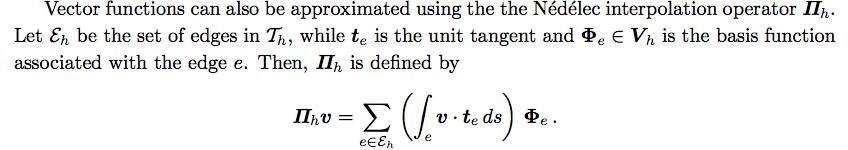
\includegraphics[width=0.9\linewidth]{Figures/P}
    \end{figure}
    \item They use the midpoint method to evaluation the integral:
    \begin{figure}[h!]
        \centering
        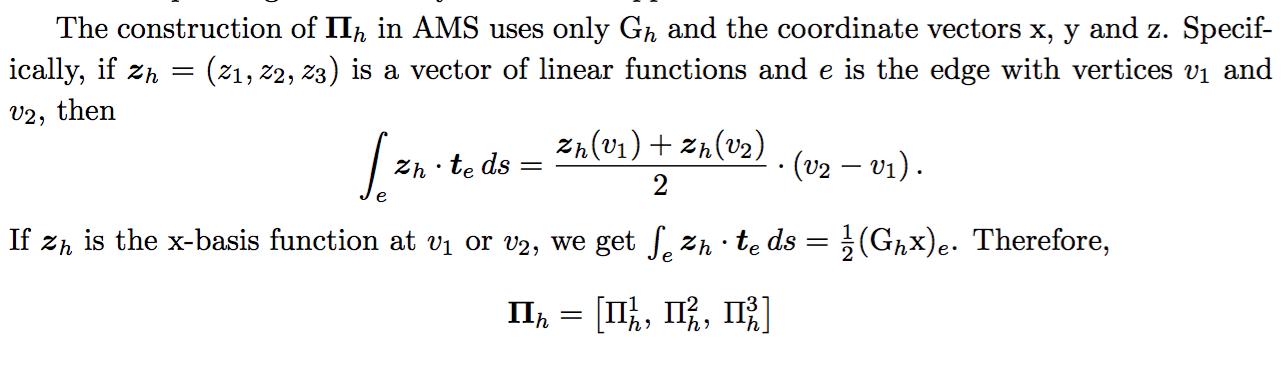
\includegraphics[width=0.9\linewidth]{Figures/Midpoint}
    \end{figure}
    \item I'm not exactly sure how you can go from the midpoint rule to either the $\frac{1}{2}(G_h \,x)_e$ ($G_h$ the discrete gradient) or your definition in \cite{LiGreif10}. Can you give any in sight?
    \item Was thinking about trying to use a similar idea for the second order elements but using Simpsons rule (or any other quadrature) to approximate the integral. Using Simpsons rule gives:
    $$ \int_e \uu{z}_h\cdot \uu{t}_e \, ds = \frac{h(\uu{z}_h(v_1) + 4 \uu{z}_h(v_1+v_2)+\uu{z}_h(v_2))}{6} \cdot (v_2-v_1) $$
    \item I'm not entirely sure exactly how to convert this into a matrix or if this is a reasonable way to proceed. Do you think this work or do you have an other ideas how to create this matrix?
    \item Using this way I do not see how the two extra degrees of freedom come into play. Do you know how these would effect the interpolation matrix?

\end{enumerate}

\begin{figure}[h!]
    \centering

    \begin{subfigure}{\textwidth}
        \centering
        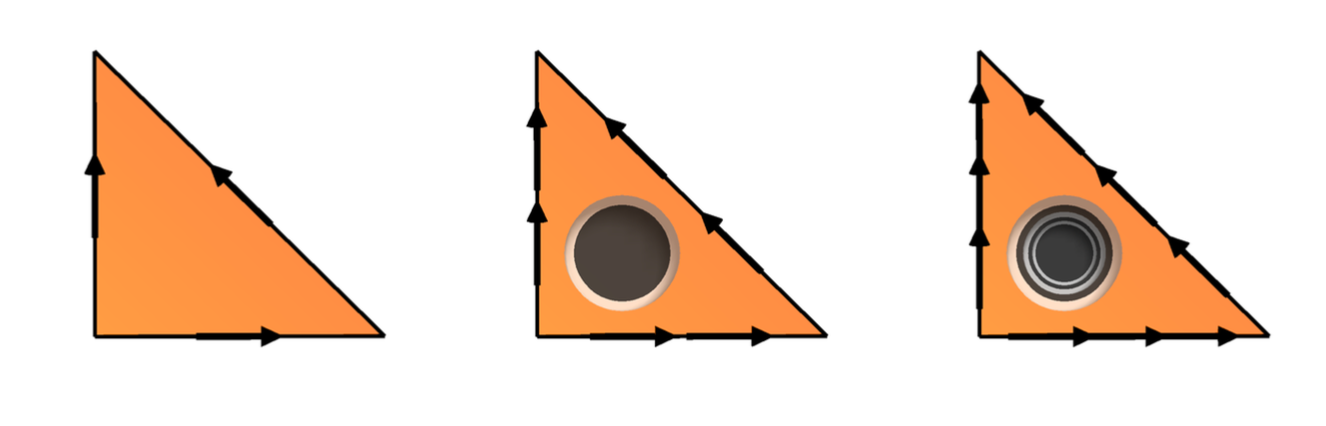
\includegraphics[width=0.4\linewidth]{Figures/Nedelec}
    \end{subfigure}

    \begin{subfigure}{\textwidth}
        \centering
        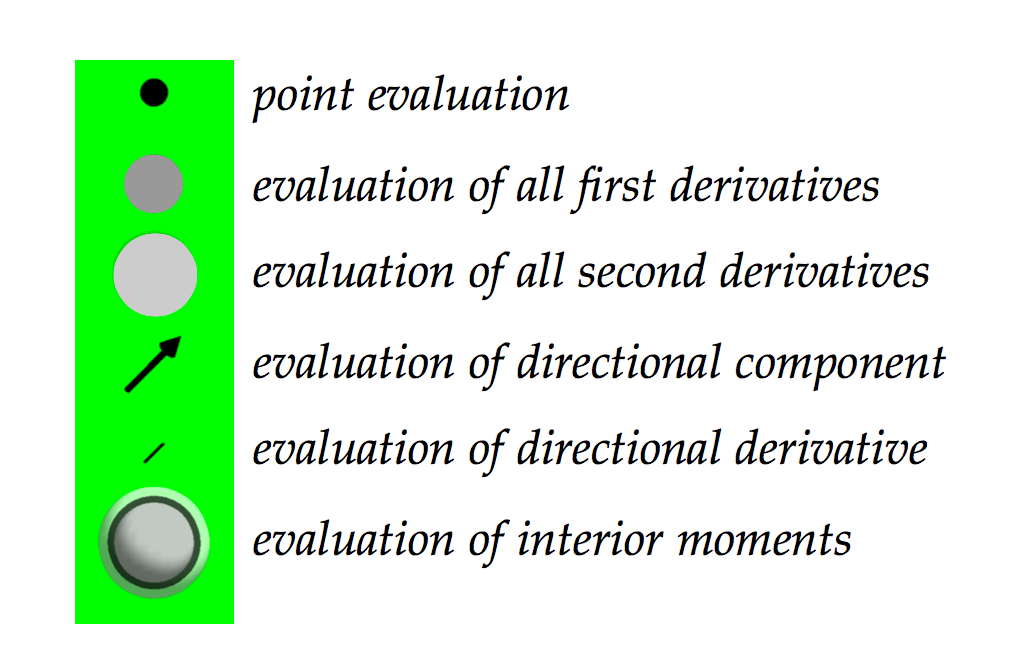
\includegraphics[width=0.4\linewidth]{Figures/DOF}
    \end{subfigure}
    \caption{\fenics DoF}
    \label{fig:fenics}

\end{figure}

For the discrete gradient matrix I can simply use the formulas in \cite{greif2007preconditioners}. I do not construct the gradient matrix explicitly but can do a mass matrix solve and a mat-vec multiplication which performs the same operation as a multiplication with the gradient matrix.

\section{Discretisation}

From an email Chen got from Scott MacLachlan (from Memorial University), they have run tests with P2/P1/N1/P1 mixed finite elements. We were not sure if he meant first order \nedelec elements as the orders of the velocity and magnetic unknowns do not match and hence were unsure if this created a stable mixed finite element.

I have run tests using this mixed finite elements and the Picard iterations do in fact converge. All the orders (presented in my thesis) match up with what we would expect apart from the $L2$ error in the velocity field, it appears to be second order instead of third.

Using this mixed element would enable us to the HX AMG method that I have already implemented for the first order elements (I still would like to understand the second order prolongation matrix). For the purposes of this paper, I think that using this element would be ok. It enables us to validate the preconditioner that we have presented (which is one of the main aspects of the paper) as well as leaving the \nedelec interpolation matrix issue alone for now.

Do you have an comments about this?



\bibliographystyle{plain}
\bibliography{refs_combine,ref_michael,ref}



\end{document}





